\section{Experimentos y evaluación}
\subsection*{Implementación del sistema}
\begin{frame}{Experimentos y evaluación}{Implementación del sistema}
\begin{itemize}
\item SPS S4 $\rightarrow$ Modifica el código fuente
	\begin{itemize}
		\item Cantidad de eventos entrantes y salientes en cada PE
	\end{itemize}
\item Distribución de la carga según la cola
	\begin{itemize}
		\item Política según el largo de la cola
	\end{itemize}
\end{itemize}

\begin{figure}
  \center
    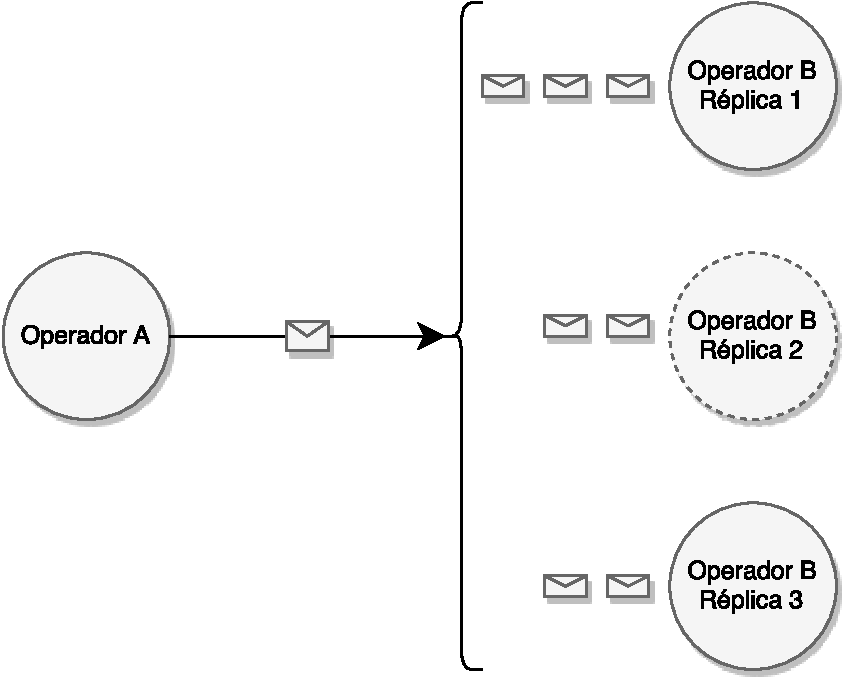
\includegraphics[scale=0.35]{images/DistribucionCarga-I.pdf}
\end{figure}
\end{frame}

\addtocounter{framenumber}{-1}
\begin{frame}{Experimentos y evaluación}{Implementación del sistema}
\begin{itemize}
\item SPS S4 $\rightarrow$ Modifica el código fuente
	\begin{itemize}
		\item Cantidad de eventos entrantes y salientes en cada PE
	\end{itemize}
\item Distribución de la carga según la cola
	\begin{itemize}
		\item Política según el largo de la cola
	\end{itemize}
\end{itemize}

\begin{figure}
  \center
    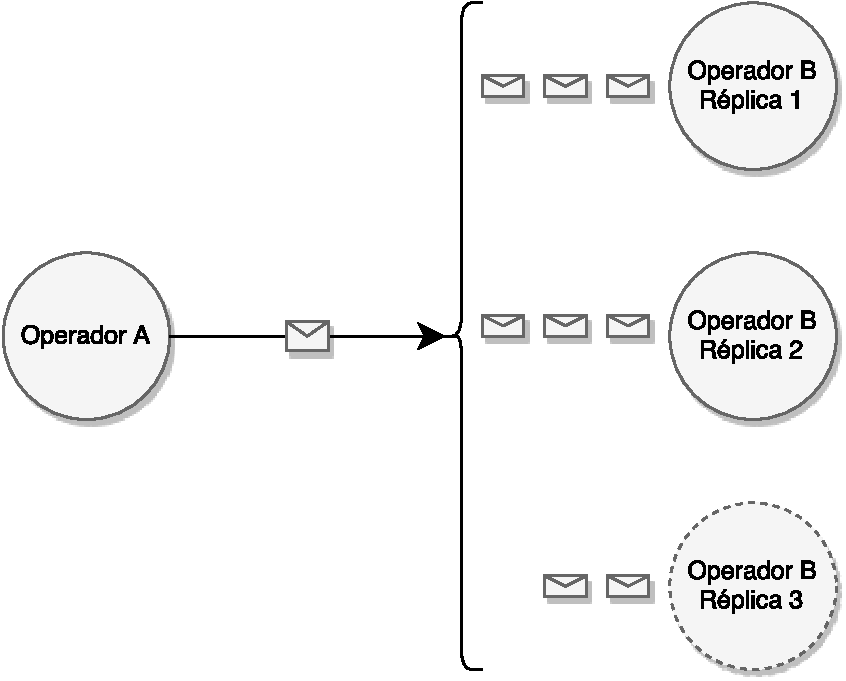
\includegraphics[scale=0.35]{images/DistribucionCarga-II.pdf}
\end{figure}
\end{frame}

\addtocounter{framenumber}{-1}
\begin{frame}{Experimentos y evaluación}{Implementación del sistema}
\begin{itemize}
\item SPS S4 $\rightarrow$ Modifica el código fuente
	\begin{itemize}
		\item Cantidad de eventos entrantes y salientes en cada PE
	\end{itemize}
\item Distribución de la carga según la cola
	\begin{itemize}
		\item Política según el largo de la cola
	\end{itemize}
\end{itemize}

\begin{figure}
  \center
    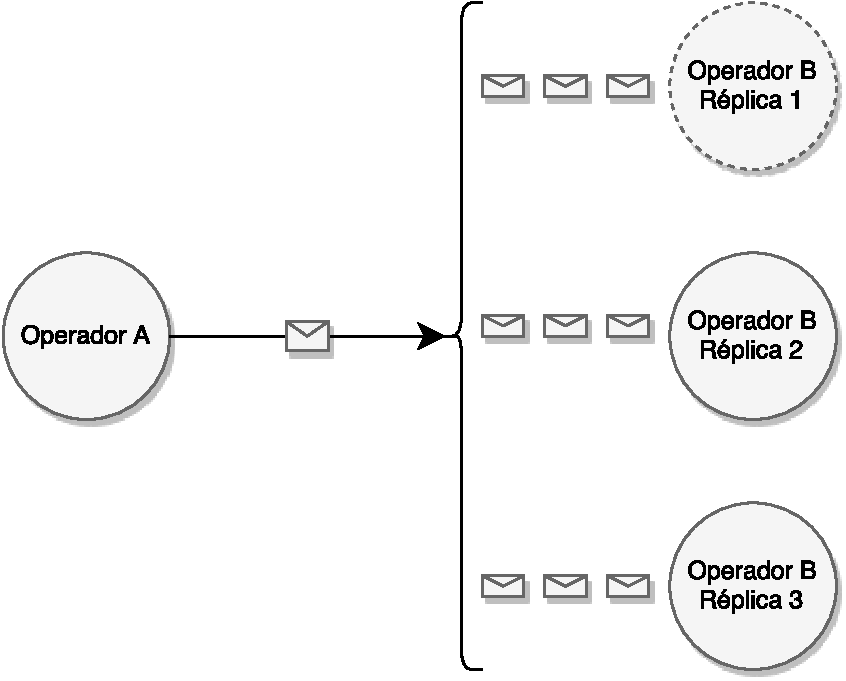
\includegraphics[scale=0.35]{images/DistribucionCarga-III.pdf}
\end{figure}
\end{frame}

\subsection*{Diseño de los experimentos}
\begin{frame}{Experimentos y evaluación}{Diseño de los experimentos}
\begin{itemize}
\item Tres tipo de aplicaciones
	\begin{itemize}
		\item Aplicación usando operadores con estado
		\item Aplicación usando operadores sin estado
		\item Aplicación sintética
	\end{itemize}
\item Generación de stream
\begin{itemize}
	\item 4.5 millones de tweets
	\item 27-28 de Febrero y 1-2 de Marzo de 2010
	\item Inglés, español y portugués
	\item Interacción entre usuarios durante el terremoto del 27 de Febrero en Chile
\end{itemize}
\end{itemize}
\end{frame}

\begin{frame}{Experimentos y evaluación}{Diseño de los experimentos}
\begin{itemize}
	\item Aplicación 1: Análisis de \textit{tweets} en escenarios de desastres naturales
\end{itemize}
\begin{figure}[!hb]
	\centering
		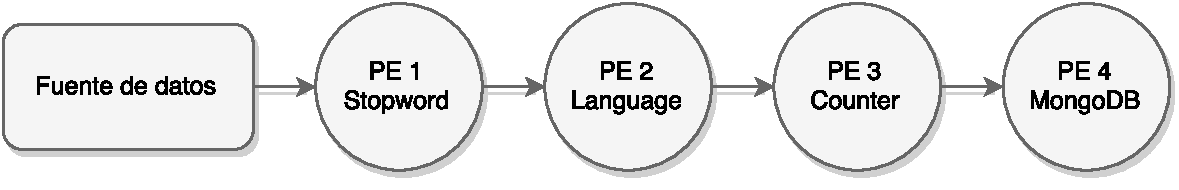
\includegraphics[scale=0.55]{images/App1.pdf}
\end{figure}
\end{frame}

\begin{frame}{Experimentos y evaluación}{Diseño de los experimentos}
\begin{itemize}
	\item Aplicación 2: Contador de palabras en muestras de textos
\end{itemize}
\begin{figure}[!ht]
	\centering
		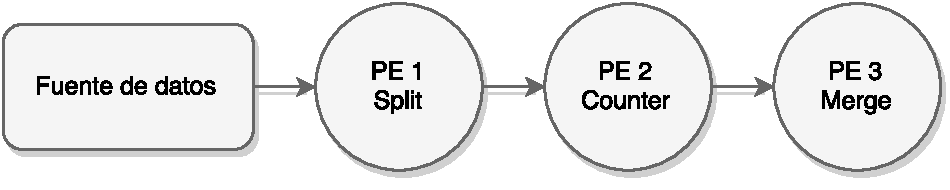
\includegraphics[scale=0.65]{images/App2.pdf}
	\label{fig:segundaAplicacion}
\end{figure}
\end{frame}

\begin{frame}{Experimentos y evaluación}{Diseño de los experimentos}
\begin{itemize}
	\item Aplicación 3: Aplicación sintética
\end{itemize}
\begin{figure}[!ht]
	\centering
		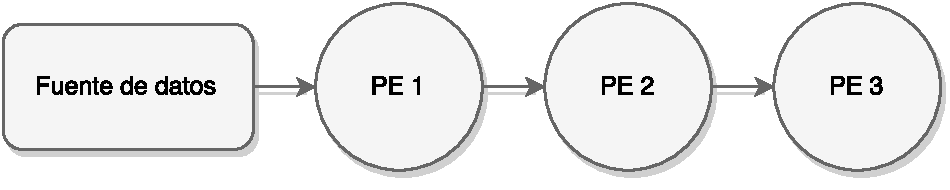
\includegraphics[scale=0.65]{images/App3.pdf}
\end{figure}
\begin{itemize}
	\item Período de tiempo que duerme la hebra asignada al PE
\end{itemize}
\begin{table}[!ht]
\footnotesize
\centering
\begin{tabular}{| c | c |}
\hline
PE & Tiempo (ms) \\ \hline
1 & 20 \\
2 & 30 \\
3 & 15 \\\hline
\end{tabular}
\end{table}
\end{frame}

\subsection*{Evaluación}
\begin{frame}{Experimentos y evaluación}{Evaluación}
\begin{itemize}
\item Para la ejecución de todos los experimentos se ha utilizado una máquina con un Intel Xeon CPU E5-2650 v2 de 2.60 GHz, 32 GB de RAM y SO Ubuntu 14.04.2 LTS

\item Para la evaluación de la primera y segunda aplicación se realiza dos tipos de experimentos
\begin{itemize}
\item Envío constante de 100 eventos/s
\item Envío variable de 50 eventos/s en primer tercio, 100 eventos/s en segundo tercio, y 50 eventos/s en último tercio
\item Ambos en un período de 70 minutos
\end{itemize}

\item Para la evaluación de la tercera aplicación se realiza un experimento
\begin{itemize}
	\item Envío constante de 100 eventos/s
	\item Período de 15 minutos
\end{itemize}

\item Cada uno de los experimentos se realiza con y sin modelo elástico

\end{itemize}
\end{frame}

%App 1%

\begin{frame}{Experimentos y evaluación}{Evaluación - App 1 - Constante - Cantidad total de eventos procesados}

\begin{itemize}
\item 401.618 eventos procesados con uso del modelo \textit{vs} 67.141 eventos procesados sin uso del modelo
\item Mejora de 6 veces la cantidad de eventos procesados
\end{itemize}

\begin{multicols}{2}
\begin{figure}[p]
	\centering
	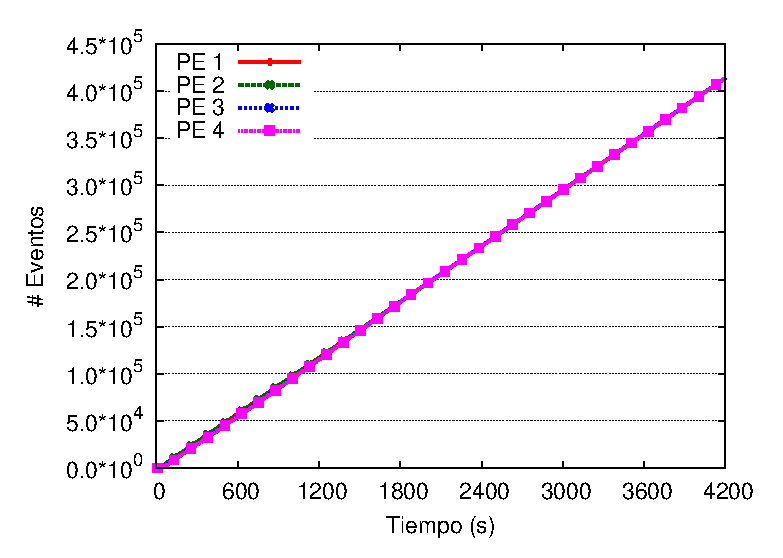
\includegraphics[scale=0.475]{images/exp/app1/uniform/cm/eventCount.eps}
\end{figure}

\begin{figure}[p]
	\centering
	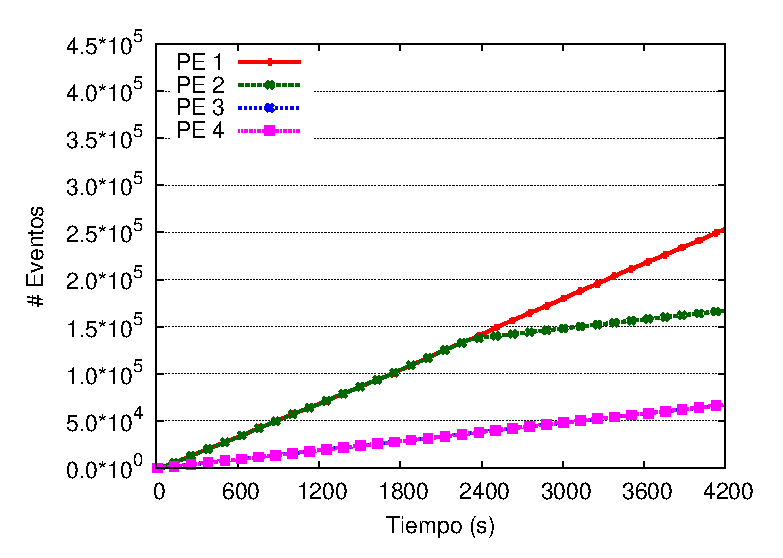
\includegraphics[scale=0.475]{images/exp/app1/uniform/sm/eventCount.eps}
\end{figure}
\end{multicols}
\end{frame}

\begin{frame}{Experimentos y evaluación}{Evaluación - App 1 - Variable - Cantidad total de eventos procesados}

\begin{itemize}
\item 303.156 eventos procesados con uso del modelo \textit{vs} 82.770 eventos procesados sin uso del modelo
\item Mejora de 3 veces la cantidad de eventos procesados
\end{itemize}

\begin{multicols}{2}
\begin{figure}[p]
	\centering
	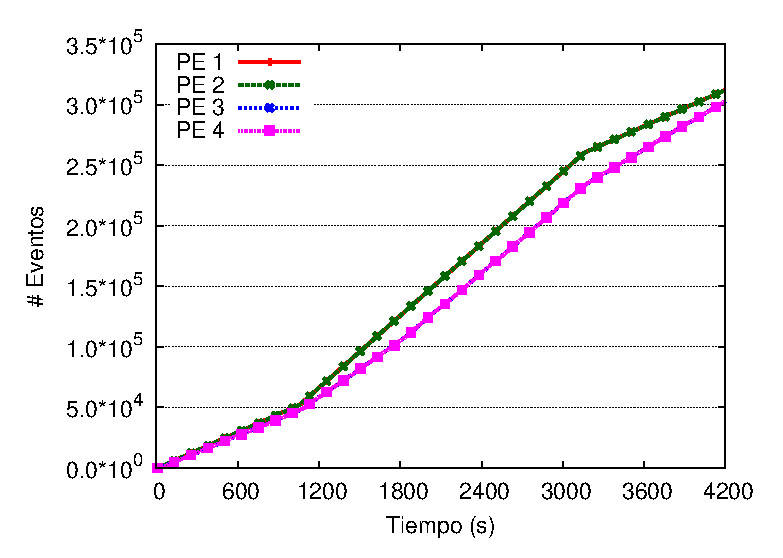
\includegraphics[scale=0.475]{images/exp/app1/normal/cm/eventCount.eps}
\end{figure}

\begin{figure}[p]
	\centering
	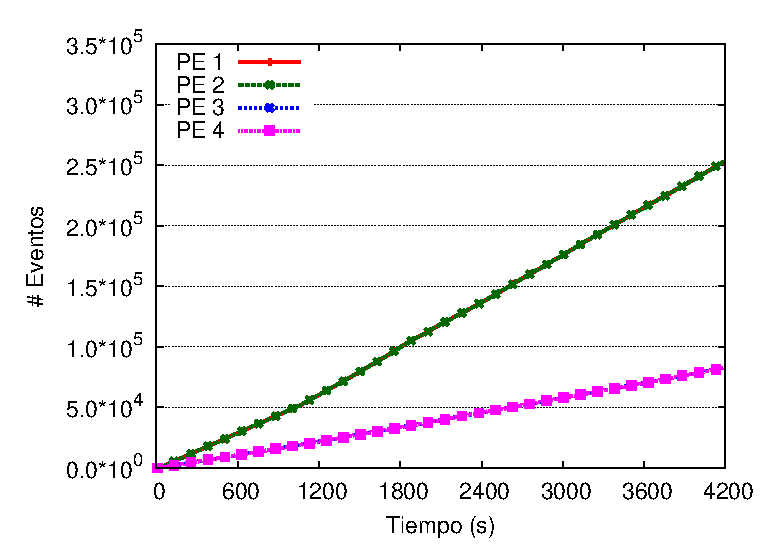
\includegraphics[scale=0.475]{images/exp/app1/normal/sm/eventCount.eps}
\end{figure}
\end{multicols}
\end{frame}

%App 2%

\begin{frame}{Experimentos y evaluación}{Evaluación - App 2 - Constante - Cantidad total de eventos procesados}

\begin{itemize}
\item 275.290 eventos procesados con uso del modelo \textit{vs} 28.152 eventos procesados sin uso del modelo
\item Mejora de 9 veces la cantidad de eventos procesados
\end{itemize}

\begin{multicols}{2}
\begin{figure}[p]
	\centering
	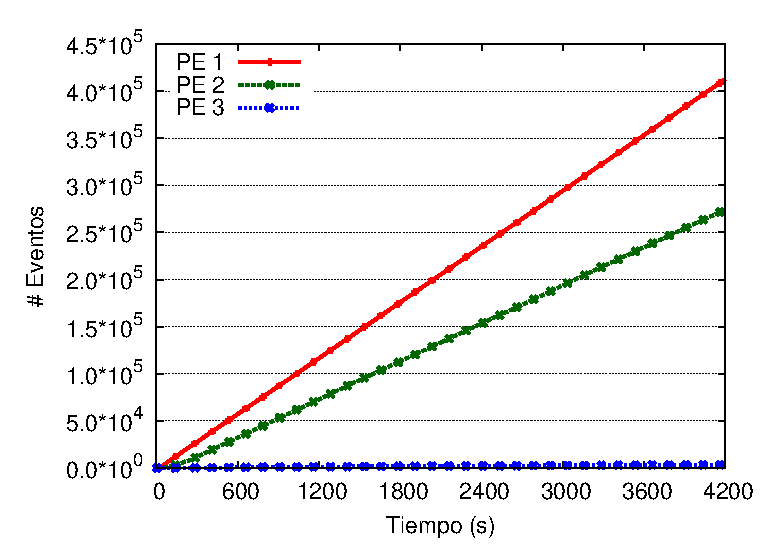
\includegraphics[scale=0.475]{images/exp/app2/uniform/cm/eventCount.eps}
\end{figure}

\begin{figure}[p]
	\centering
	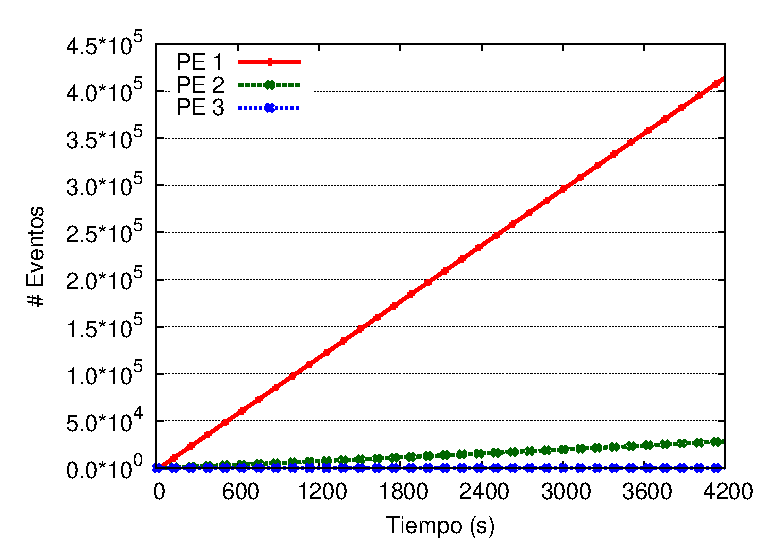
\includegraphics[scale=0.475]{images/exp/app2/uniform/sm/eventCount.eps}
\end{figure}
\end{multicols}
\end{frame}

\begin{frame}{Experimentos y evaluación}{Evaluación - App 2 - Variable - Cantidad total de eventos procesados}

\begin{itemize}
\item 228.942 eventos procesados con uso del modelo \textit{vs} 27.751 eventos procesados sin uso del modelo
\item Mejora de 8 veces la cantidad de eventos procesados
\end{itemize}

\begin{multicols}{2}
\begin{figure}[p]
	\centering
	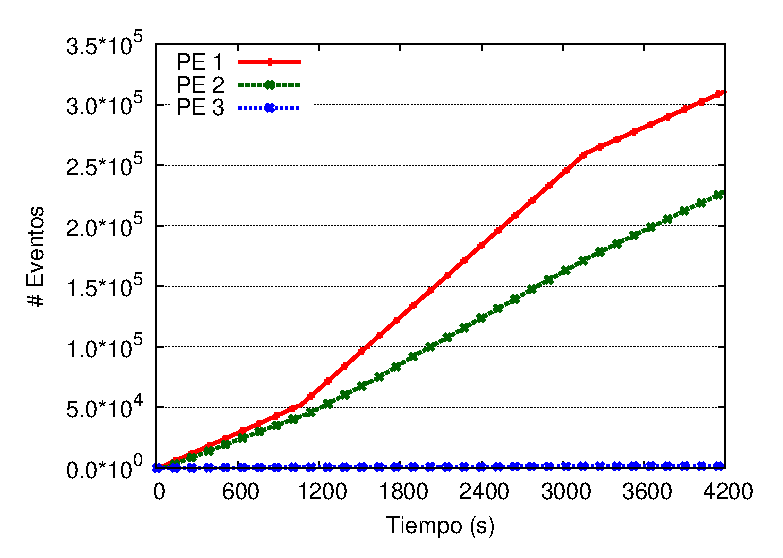
\includegraphics[scale=0.475]{images/exp/app2/normal/cm/eventCount.eps}
\end{figure}

\begin{figure}[p]
	\centering
	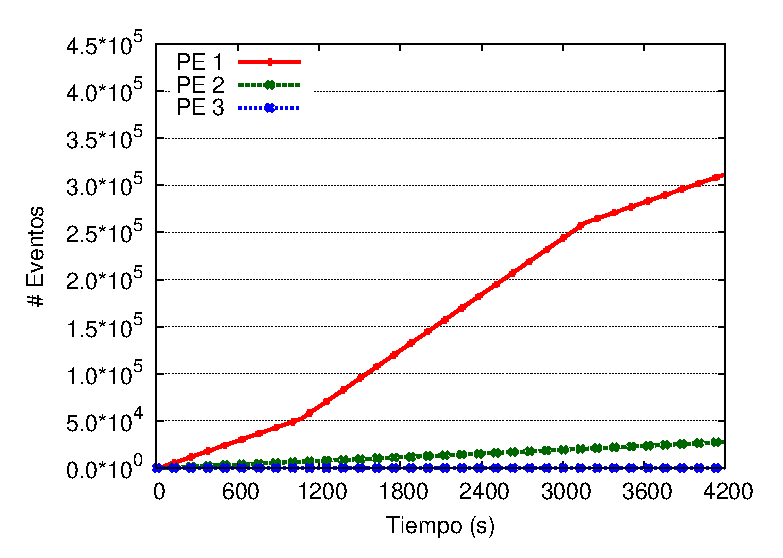
\includegraphics[scale=0.475]{images/exp/app2/normal/sm/eventCount.eps}
\end{figure}
\end{multicols}
\end{frame}

\begin{frame}{Experimentos y evaluación}{Evaluación - App 3 - Constante - Utilización promedio de CPU}

\begin{itemize}
\item $0,62\%$ con uso del modelo \textit{vs} $0,61\%$ sin uso del modelo
\item Aumento de un $0,01\%$ de utilización promedio de CPU
\end{itemize}

\begin{multicols}{2}
\begin{figure}[p]
	\centering
	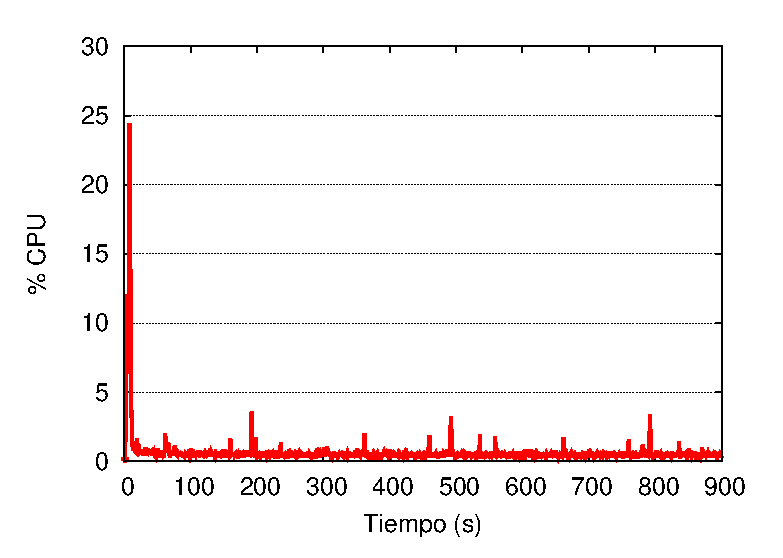
\includegraphics[scale=0.475]{images/exp/app3/cm/fisical/consumeCPU.eps}
\end{figure}

\begin{figure}[p]
	\centering
	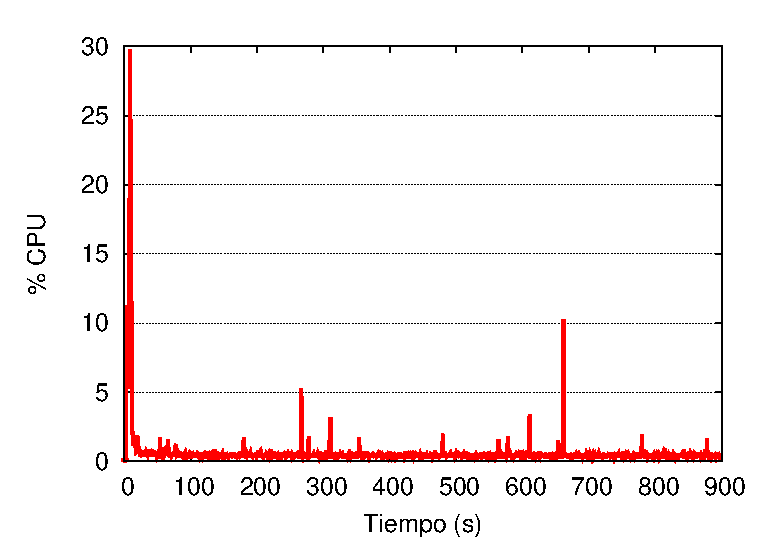
\includegraphics[scale=0.475]{images/exp/app3/sm/fisical/consumeCPU.eps}
\end{figure}
\end{multicols}
\end{frame}

\begin{frame}{Experimentos y evaluación}{Evaluación - App 3 - Constante - Consumo de memoria RAM}

\begin{itemize}
\item $264$MB con uso del modelo \textit{vs} $268$MB sin uso del modelo
\item Disminución de $1,5\%$ de consumo de memoria RAM
\end{itemize}

\begin{multicols}{2}
\begin{figure}[p]
	\centering
	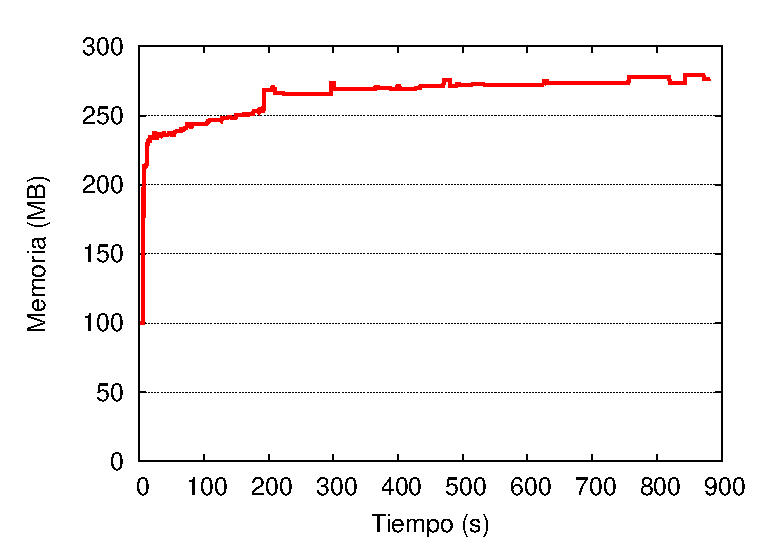
\includegraphics[scale=0.475]{images/exp/app3/cm/fisical/consumeRAM.eps}
\end{figure}

\begin{figure}[p]
	\centering
	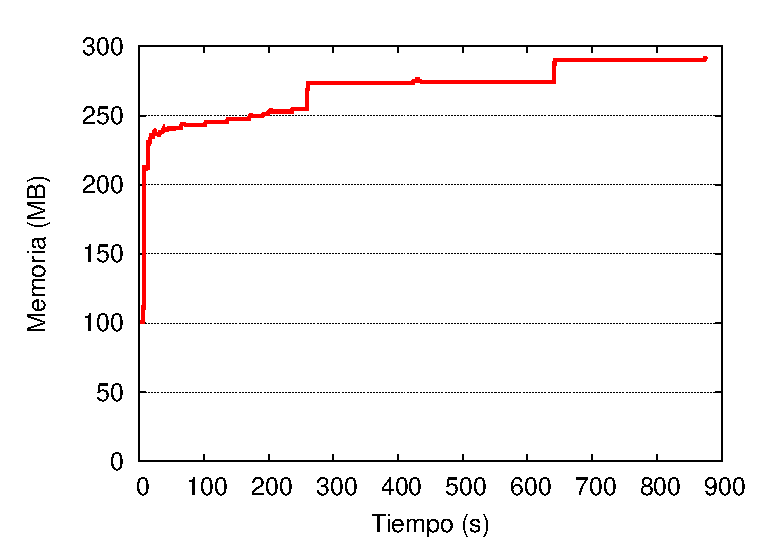
\includegraphics[scale=0.475]{images/exp/app3/sm/fisical/consumeRAM.eps}
\end{figure}
\end{multicols}
\end{frame}

\begin{frame}{Experimentos y evaluación}{Evaluación - App 3 - Constante - Cantidad total de eventos procesados}

\begin{itemize}
\item 88.169 eventos procesados con uso del modelo \textit{vs} 28.714 eventos procesados sin uso del modelo
\item Mejora de 3 veces la cantidad de eventos procesados
\end{itemize}

\begin{multicols}{2}
\begin{figure}[p]
	\centering
	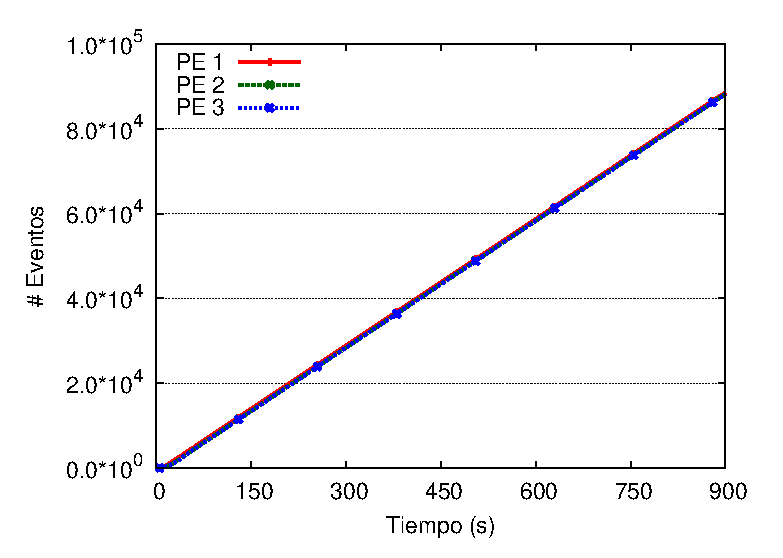
\includegraphics[scale=0.475]{images/exp/app3/cm/logical/eventCount.eps}
\end{figure}

\begin{figure}[p]
	\centering
	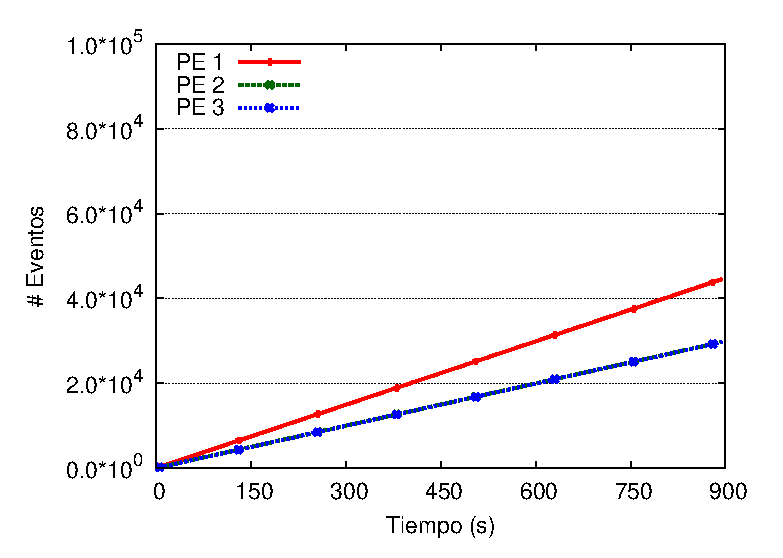
\includegraphics[scale=0.475]{images/exp/app3/sm/logical/eventCount.eps}
\end{figure}
\end{multicols}
\end{frame}

\begin{frame}{Conclusiones}{Detalles de la contribución}

\begin{itemize}
\item Diseño e implementación de un modelo elástico
\begin{itemize}
	\item Algoritmo reactivo
	\item Algoritmo predictivo
	\item Módul de administración de réplicas
\end{itemize}
\item Construcción de tres escenarios $\rightarrow$ Validación del modelo diseñado
\item Evaluado y analizado el rendimiento del sistema con y sin uso del modelo elástico
\end{itemize}

\end{frame}